\chapter{Risultati sperimentali}

In questo capitolo verranno esposti i risultati che sono stati trovati
utilizzando il dataset \textit{Aquaint} e il relativo test set.

\section{Valori di riferimento}
Come prima cosa è necessario capire sul dataset in questione
quali sono le prestazioni ottenibili utilizzando l'algoritmo rivale di BM25P,
BM25. I seguenti risultati sono stati calcolati con gli iperparametri standard
di BM25.

\begin{table}[h!]
	\centering
	\begin{tabular}{|c|c|}
		\hline
		recall@100 & 0.2071 \\
		\hline
		recall@200 & 0.3069 \\
		\hline
		NDCG & 0.4161 \\
		\hline
		NDCG@5 & 0.2800 \\
		\hline
		NDCG@10 & 0.2707 \\
		\hline
	\end{tabular}
\caption{Valutazione di BM25}
\end{table}

Con la notazione $misura@k$ si intende che
la misura è stata effettuata sui primi $k$ risultati, in gergo tecnico
è chiamato taglio.

\section{Algoritmo Grid Search}
Utilizzando l'agoritmo Grid Search con i seguenti valori:

\begin{table}[h!]
	\centering
	\begin{tabular}{|c|c|}
		\hline
		$w_{start}$ & $[0.5, 0.5, 0.5, 0.5, 0.5, 0.5, 0.5, 0.5, 0.5, 0.5]$ \\
		\hline
		$w_{end}$ & $[5.0, 5.0, 5.0, 5.0, 5.0, 5.0, 5.0, 5.0, 5.0, 5.0]$ \\		
		\hline
		$w_{step}$ & 0.25 \\
		\hline
	\end{tabular}
\caption{Configurazione di GridSearch}
\end{table}

I valore massimi delle funzioni di valutazione trovati
sono i seguenti:

\begin{table}[h!]
	\centering
	\begin{tabular}{|c|c|}
		\hline 
		recall@100  &  0.1932  \\
		\hline
		recall@200   & 0.2786 \\
		\hline
		NDCG    & 0.3845 \\
		\hline
		NDCG@5  & 0.3246 \\
		\hline
		NDCG@10  & 0.2952 \\
		\hline
		\multicolumn{2}{|c|}{$w = [1.531, 0.843, 0.863, 0.861, 0.856 , 0.912, 0.874, 0.856, 0.865, 1.534]$} \\
		\hline
	\end{tabular}
	\caption{Risultati di GridSearch}
\end{table}

\begin{figure}[h!]
	\centering
	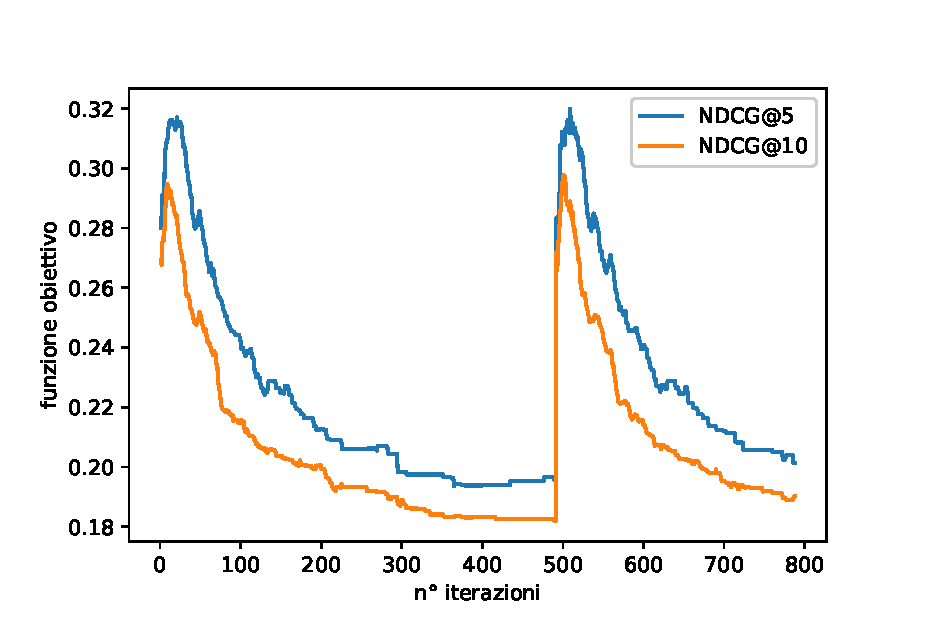
\includegraphics[width=0.7\linewidth]{figure/gs_search}
	\caption[Andamento della funzione obiettivo utilizzando GridSearch]{}
	\label{fig:gssearch}
\end{figure}


Grid Search dopo svariate ore di lavoro non è riuscito a produrre risultati soddisfacenti.

\section{Line Search with Random Restart}

\begin{table}[h!]
	\centering
	\begin{tabular}{|c|c|}
		\hline
		recall@100 &  0.1988 \\
		\hline
		recall@200 & 0.2793  \\
		\hline
		NDCG & 0.3814 \\
		\hline
		NDCG@5 & 0.3188 \\
		\hline
		NDCG@10 & 0.2901 \\
		\hline
		\multicolumn{2}{|c|}{
			$w = [1.071, 0.821, 0.821, 0.821, 0.821, 0.821, 1.071, 0.821, 1.0714, 1.071]$ 
		} \\
	\hline
	\end{tabular}
	\caption{Risultati di Line Search with Random Restart}
\end{table}

\section{Increase Search}

\begin{table}[h!]
	\centering
	\begin{tabular}{|c|c|}
		\hline
		recall@100 &  0.1971  \\
		\hline
		recall@200 & 0.2954  \\
		\hline
		NDCG & 0.4119 \\
		\hline
		NDCG@5 & 0.3542 \\
		\hline
		NDCG@10 & 0.3007 \\
		\hline
		\multicolumn{2}{|c|}{$w = [0.1981, 0.1012, 0.07532, 0.075321, 0.15023, 0.12532, 0.12512, 0.103, 0.0521, 0.2534]$} \\
		\hline
	\end{tabular}
	\caption{Risultati di Increase Search}
\end{table}

\section{Risultati}

Com'è possibile notare il vettore dei pesi migliore è quello che è stato trovato
dall'algoritmo Increase Search, producendo un incremento del $7\%$  rispetto all'orginale BM25.
Pertanto tale algoritmo, avendo a disposizione di un budget di tempo $\mathcal{B}$ nell'ordine
delle ore, performa maggiormente rispetto agli altri.
Ovviamente aumentando $\mathcal{B}$ diventa possibile utilizzare anche gli altri
tipi di algoritmi, quali Grid Search o Line Search with Random Restart.

\section{Test di significatività statistico}

Prima di poter concludere che BM25P con il $w$ ottimo è migliore di BM25, è necessario
fare un test statistico, il cui obiettivo è quello di capire se $\text{BM25P}_w$ $\equiv$ BM25
cioè se essi sono uguali.

Il test è chiamato test di significatività statistico, il quale obiettivo
è quello di capire se due medie provengono da distribuzioni diverse oppure no.
Inannzitutto si deve formulare la \textit{null-hypothesis}, cioè l'ipotesi
della quale vogliamo provarne la falsità.

\begin{esempio}
	Si lancia un dado 10 volte e si calcola la media $\bar{X}_2$. Dopo un giorno si ripete l'esperimento
	e si ricalcola la media $\bar{X}_2$. Molto probabilmente si noterà che $\bar{X}_1 \neq \bar{X}_2$,
	ma tali valori provengono da distrubuzioni diverse?
	Ovviamente no, poiché i dadi sono gli stessi, dunque se la null-hypothesis fosse
	stata $X_1 \equiv X_2$, allora avremmo potuto renderla vera.
\end{esempio}

Dunque in questo caso siamo in grado accetare l'ipotesi perché
sapevamo già a priori che le due distribuzioni erano uguali, ma nel caso
in cui non lo sapessimo?
Uno dei modi più veloci di giudicare la null-hypothesis è quello di eseguire un test statistico.
Accordandoci con l'articolo\cite{10.1145/1321440.1321528}, il miglior test per valutare
due ranker è quello chiamato \textit{Fisher's Randomization Test}.

\subsection{Il test Randomizzato di Fisher}
Tale test si basa sull'ipotizzare che due ranker $\mathcal{R}_1 $ e $\mathcal{R}_2$ siano identici
e che un altro ranker $\mathcal{R}_F$ si impossessi dei risultati di entrambi e
ritorni casualmente o quello di uno o quello di un altro.
Il ruolo giocato da $\mathcal{R}_F$ è di fondamentale importanza, poiché esso produce un risultato
casuale tra i due, pertanto, se essi fossero identici la distrubuzione non cambierebbe.
Ma l'obiettivo principale è quello di calcolare la probabilità che la differenza
di performance tra i due è soltanto dovuta al fatto che $\mathcal{R}_3$ sceglie casualmente
il risultato tra i due ranker.

Per eseguire il test ipotizziamo di avere a disposizione un dataset formato da una lista
di coppie $\langle e_{A}, e_{B}\rangle$, dove la lettera $e$ indica la funzione di valutazione
scelta: nel caso in questione NDCG@5. I pedici $A$ e $B$ indicano invece rispettivamente i due
ranker, dove per semplicità di trattazione abbiamo posto che $A$ è BM25P e $B$ è BM25. Tali valutazioni sono calcolate solo e soltanto su una query,
pertanto abbiamo a disposizione 50 coppie.

\paragraph{Definizioni}
Definiamo le seguenti quantità:

\begin{itemize}
	\item $N$ la lunghezza della lista del dataset (nel caso in questione $N=50$)
	\item $\sigma_A = \sum_{i=1}^{N} e_{A_i}$ e $\sigma_B = \sum_{i=1}^{N} e_{B_i}$
	\item $\bar{e}_A = \frac{\sigma_{A} }{N}$ e  $\bar{e}_B = \frac{\sigma_{B} }{N}$, cioè le relative medie aritmetiche
	\item $d = \sigma_{A} - \sigma_{B}$, cioè la differenza di performance tra i due ranker
\end{itemize}


\begin{algorithm}[h!]
	\SetAlgorithmName{Algoritmo}{}
	\small
	\DontPrintSemicolon
	\SetKwInOut{Input}{Input}
	\SetKwInOut{Output}{Output}
	\Input{$e_A$ lista delle valutazioni del ranker A}
	\Input{$e_B$ lista delle valutazioni del ranker B}
	\Input{$d$}
	\Input{$k$}
	\Input{$\sigma_A, \sigma_B$}
	\Input{$\bar{e}_A, \bar{e}_B$}
	\Output{$p_1,p_2$}
	\BlankLine
	$p_1 = 0, p_2 = 0$\;
	\BlankLine
	\For{$i=1$ \textbf{to} $k$}{
		$a,b = \text{randomChoice}(e_A, e_B)$\;
		$\bar{a} = avg(a)$\;
		$\bar{b} = avg(b)$\;
		
		\BlankLine
		$\delta = \bar{a} - \bar{b}$\;
		\If{$\delta \geq d$}{
			$p_1 = p_1 + 1$\;
		}
		\If{$\left|\delta\right| \geq \left|d\right|$}{
			$p_2 = p_2 + 1$\;
		}
	}
	
	\Return{$\frac{p_1}{k}, \frac{p_2}{k}$}
	\label{alg:spectest}
	\caption{Algoritmo per l'esecuzione del test di randomizzazione di Fisher}
\end{algorithm}

A questo punto si procede scegliendo un numero massimo $k$ di permutazioni
da eseguire, poichè  senza limitazioni  il test avrebbe complessità $\mathcal{O}(2^N)$
e dunque per valori di $N$ elevati ci vorrebbe troppo tempo per eseguirlo.
\\
\\
Successivamente l'algoritmo esegue un ciclo, scorrendo un indice fino ad arrivare a $k$.
Nel corpo del ciclo, essoo prende a caso un elemento della lista di $e_A$ o di $e_B$ e
calcola la differenza di qualità ottenuta.
A seconda dei risultati vengono incrementi i valori $p_1$ o $p_2$, che costituiscono
l'output dell'algoritmo stesso.

Riassumendo, ciò che $\mathcal{R}_3$ esegue è un assegnamento casuale di etichette e
possiamo considerare Il test valido se la scelta è casuale (anche se in questo caso
dobbiamo accontentarci della pseudocasualità).

\paragraph{Il risultato del test}
I valori calcolati dall'algoritmo, cioè $p_1$ e $p_2$, sono due rapporti:

\begin{itemize}
	\item $p_1$ è detto anche ``one-sided-p-value", ovvero il rapporto tra il numero di volte che la differenza
	della valutazione è più grande di quella ipotizzata e il numero di permutazioni
	\item $p_2$ è detto invece ``two-sided-p-value", overo il solito significato di $p_1$ ma utilizzando
	come metrica di differenza il valore assoluto.
\end{itemize}


Per poter valutare dunque la veridicità della \textit{null-hypothesis} si usano tali valori,
cioè $p_1$ e $p_2$ costituiscono un'approssimazione della probabilità che che i due ranker
siano uguali. Solitamente si sceglie un valore $\alpha < 0.05$ per cui si valuta che
se $p_1$ e $p_2$ sono maggiori di $\alpha$ allora l'ipotesi non può essere rifiutata,
mentre se sono minori l'ipotesi è falsa, e dunque i due ranker sono diversi.


\subsection{Esecuzione nel caso di BM25P}
L'esperimento è stato condotto sul solito dataset, isolando le query tal topic file e calcolando la NDCG
per ogni ogni query, sia con BM25P che con BM25P.

Il test ha riportato i seguenti valori

\begin{table}[h!]
	\centering
	\begin{tabular}{|c|c|c|}
		\hline
		\textbf{Misura} & $p_1$ & $p_2$ \\
		\hline
		NDCG  & 0.13218 & 0.26347 \\
		\hline
		NDCG@5 & 0.00082 & 0.00145 \\
		\hline
		NDCG@10 & 0.03454 & 0.06835 \\
		\hline
	\end{tabular}
	\caption{Risultati del test statistico su BM25P}
\end{table}

Considerando i valori standard di $\alpha$, la \textit{null-hypothesis} (BM25P $\equiv$ BM25) può essere considerata falsa.
Questo perché, dato che l'ottimizzazione di BM25P è stata basata sui tagli più piccoli, il test di significatività statistico su NDCG@5 e NDCG@10 
deve avere più peso rispetto a NDCG senza tagli.
Questo risultato inoltre ci mostra che i due ranker, su tagli più grandi, potrebbero essere simili, in quanto $p_2 > p_1 > \alpha$. \footnote{Potrei aggiungere all'appendice anche lo snippet in python?}
